\chapter{Các kỹ thuật liên quan}
Trong chương này, khóa luận trình bày chi tiết cơ sở lý thuyết và các nghiên cứu liên quan trực tiếp làm nền tảng phát triển phương pháp đề xuất: (1) Kiến trúc nền tảng đa phương thức \textbf{LayoutLMv3} \cite{huang2022layoutlmv3} cho bài toán hiểu tài liệu giàu thị giác; (2) Các hướng tiếp cận mô hình hóa cấu trúc hình học và ngữ cảnh phân đoạn trong Document AI; và (3) Phân tích xung đột độ mịn giữa cấp độ token và cấp độ phân đoạn trong bài toán KIE discriminative.

\section{Mô hình nền tảng đa phương thức LayoutLMv3}
LayoutLMv3 \cite{huang2022layoutlmv3}, được đề xuất bởi Huang và cộng sự tại hội nghị ACM Multimedia 2022, là mô hình nền tảng đa phương thức tiêu biểu nhất cho các tác vụ Document AI. Khác với các thế hệ tiền nhiệm như LayoutLMv2 \cite{xu2021layoutlmv2} hay DocFormer \cite{appalaraju2021docformer} vốn phụ thuộc vào mạng xương sống thị giác CNN phức tạp (như ResNeXt-101-FPN) và quy trình phát hiện vùng ảnh tốn kém, LayoutLMv3 sử dụng một bộ mã hóa Transformer hợp nhất duy nhất nhận đầu vào trực tiếp là các token văn bản kết hợp với chuỗi mảnh ảnh tuyến tính. Tổng quan kiến trúc và các mục tiêu tiền huấn luyện của LayoutLMv3 được minh họa trong Hình \ref{fig:layoutlmv3_arch}.

\begin{figure}[htbp]
    \centering
    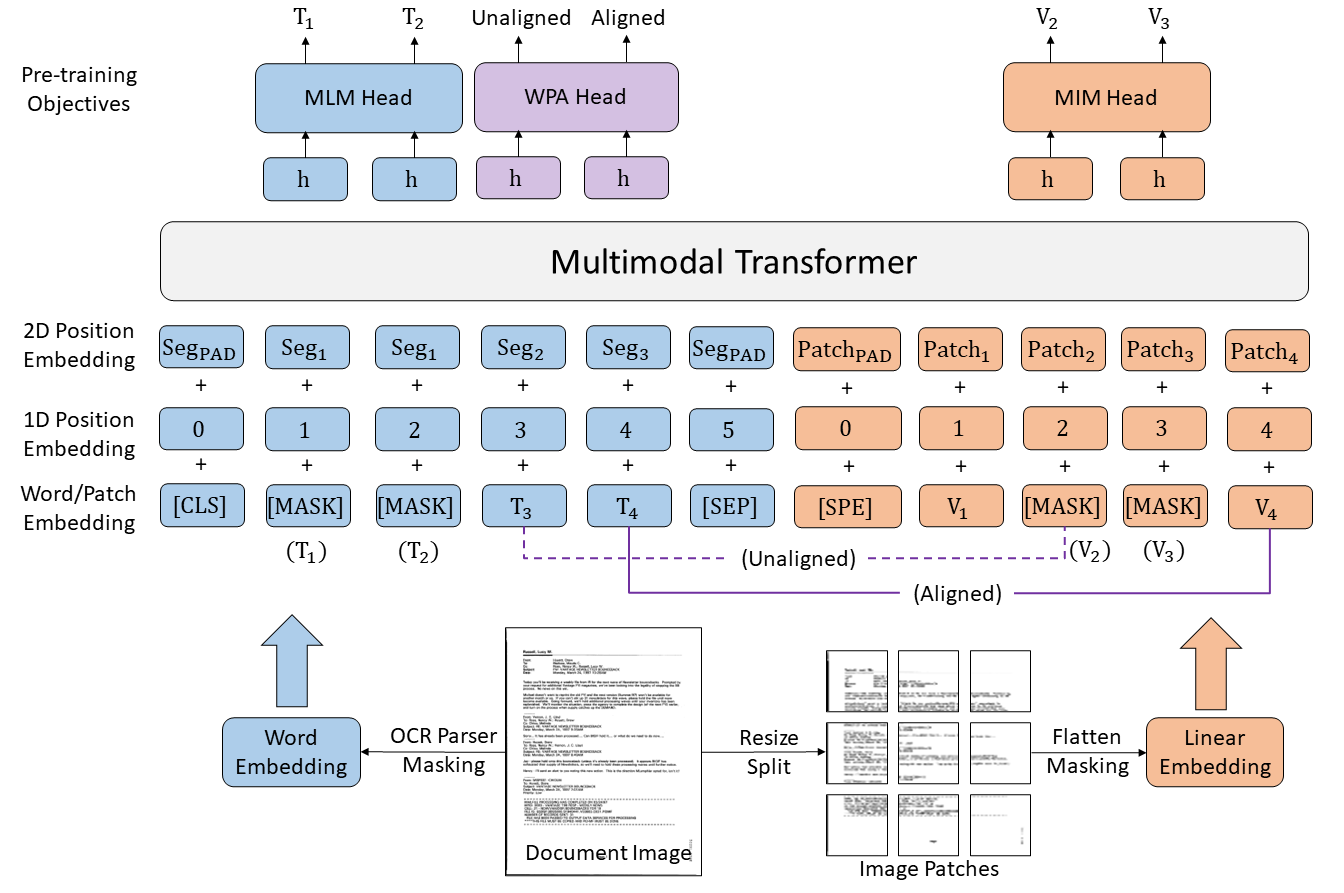
\includegraphics[width=0.95\linewidth]{chapter2/architecture.png}
    \caption{Kiến trúc tổng thể và các mục tiêu tiền huấn luyện hợp nhất của mô hình LayoutLMv3 \cite{huang2022layoutlmv3}.}
    \label{fig:layoutlmv3_arch}
\end{figure}

\subsection{Biểu diễn nhúng văn bản và không gian hai chiều}
Đối với kênh văn bản, mỗi tài liệu được biểu diễn bởi chuỗi gồm $L$ token sau khi phân tách từ bằng bộ từ vựng Byte-Level BPE (tương tự RoBERTa). Với mỗi token thứ $i \in \{1, \dots, L\}$, biểu diễn nhúng cơ sở $\mathbf{e}_i^{\text{base}} \in \mathbb{R}^{d_{\text{model}}}$ (trong đó $d_{\text{model}} = 768$ đối với bản \texttt{base} và $d_{\text{model}} = 1024$ đối với bản \texttt{large}) được tổng hợp từ ba thành phần:
\begin{enumerate}
    \item \textbf{Nhúng từ vựng:} $\mathbf{e}_i^{\text{word}} = \mathbf{E}_{\text{word}}(t_i) \in \mathbb{R}^{d_{\text{model}}}$ ánh xạ mã định danh từ vựng $t_i$ sang không gian véc-tơ liên tục.
    \item \textbf{Nhúng vị trí một chiều:} $\mathbf{e}_i^{\text{1D}} = \mathbf{E}_{\text{pos1D}}(i) \in \mathbb{R}^{d_{\text{model}}}$ biểu diễn thứ tự tuần tự của token trong chuỗi đầu vào.
    \item \textbf{Nhúng vị trí không gian hai chiều:} Thay vì gán tọa độ riêng lẻ cho từng từ con, LayoutLMv3 áp dụng cơ chế bố cục mức phân đoạn: các từ cùng thuộc một dòng/phân đoạn OCR chia sẻ chung một hộp giới hạn bao quanh $\mathbf{b}_i = (x_0, y_0, x_1, y_1) \in [0, 1000]^4$ cùng chiều rộng $w = \text{clip}(x_1 - x_0, 0, 1023)$ và chiều cao $h = \text{clip}(y_1 - y_0, 0, 1023)$. Sáu giá trị hình học này được tra cứu qua các bảng nhúng tọa độ $\mathbf{E}_x, \mathbf{E}_y \in \mathbb{R}^{1024 \times d_{\text{coord}}}$ và bảng nhúng kích thước $\mathbf{E}_w, \mathbf{E}_h \in \mathbb{R}^{1024 \times d_{\text{shape}}}$ rồi ghép nối lại thành véc-tơ không gian $\mathbf{e}_i^{\text{2D}} \in \mathbb{R}^{d_{\text{model}}}$:
    \begin{equation}
        \label{eq:spatial_2d_emb}
        \mathbf{e}_i^{\text{2D}} = \left[ \mathbf{E}_x(x_0) \;\Vert\; \mathbf{E}_y(y_0) \;\Vert\; \mathbf{E}_x(x_1) \;\Vert\; \mathbf{E}_y(y_1) \;\Vert\; \mathbf{E}_h(h) \;\Vert\; \mathbf{E}_w(w) \right],
    \end{equation}
    với $4 d_{\text{coord}} + 2 d_{\text{shape}} = d_{\text{model}}$ (cụ thể trong \texttt{layoutlmv3-base}, $d_{\text{coord}} = 128, d_{\text{shape}} = 128 \Rightarrow 4 \times 128 + 2 \times 128 = 768$).
\end{enumerate}

Khi đó, véc-tơ nhúng văn bản chuẩn hóa của token thứ $i$ (cài đặt trong lớp \texttt{LayoutLMv3Embeddings}) được tính bởi công thức:
\begin{equation}
    \label{eq:base_text_emb}
    \mathbf{x}_i^{\text{text}} = \text{Dropout}\!\left(\text{LayerNorm}\!\left(\mathbf{e}_i^{\text{word}} + \mathbf{e}_i^{\text{type}} + \mathbf{e}_i^{\text{1D}} + \mathbf{e}_i^{\text{2D}}\right)\right),
\end{equation}
trong đó $\mathbf{e}_i^{\text{type}}$ là nhúng kiểu token (mặc định bằng $\mathbf{0}$).

\subsection{Biểu diễn nhúng mảnh ảnh thị giác}
Đối với kênh hình ảnh, ảnh tài liệu $\mathcal{I}$ được thay đổi kích thước về $H_{\text{img}} \times W_{\text{img}} = 224 \times 224$ và chuẩn hóa theo trung bình và độ lệch chuẩn của ImageNet Inception. Mô-đun \texttt{PatchEmbed} chia ảnh thành lưới các mảnh vuông không giao nhau kích thước $P \times P = 16 \times 16$, tạo ra $M_{\text{img}} = \frac{224}{16} \times \frac{224}{16} = 14 \times 14 = 196$ mảnh ảnh. Một phép tích chập hai chiều $\text{Conv2d}(3, d_{\text{model}}, \text{kernel\_size}=16, \text{stride}=16)$ chiếu tuyến tính từng mảnh ảnh sang không gian $d_{\text{model}}$, sau đó cộng với nhúng vị trí ảnh 1D học được và ghép thêm 1 token phân loại thị giác $\texttt{[CLS]}_{\text{vis}}$ ở đầu chuỗi, thu được tổng cộng $M_{\text{vis}} = 197$ token thị giác:
\begin{equation}
    \label{eq:visual_tokens}
    \mathbf{X}^{\text{vis}} = \left[ \mathbf{x}_{\text{CLS}}^{\text{vis}}, \mathbf{x}_1^{\text{vis}}, \dots, \mathbf{x}_{196}^{\text{vis}} \right] \in \mathbb{R}^{197 \times d_{\text{model}}}.
\end{equation}

Chuỗi văn bản $\mathbf{X}^{\text{text}} \in \mathbb{R}^{L \times d_{\text{model}}}$ và chuỗi thị giác $\mathbf{X}^{\text{vis}} \in \mathbb{R}^{197 \times d_{\text{model}}}$ được ghép nối dọc theo chiều độ dài chuỗi thành chuỗi đa phương thức hợp nhất $\mathbf{H}^{(0)} = [\mathbf{X}^{\text{text}} \;\Vert\; \mathbf{X}^{\text{vis}}] \in \mathbb{R}^{(L + 197) \times d_{\text{model}}}$ để đưa vào bộ mã hóa Transformer.

\subsection{Cơ chế tự chú ý nhận thức không gian và ổn định hóa CogView}
Bộ mã hóa của LayoutLMv3 gồm $N_{\text{layer}}$ lớp Transformer xếp chồng ($N_{\text{layer}} = 12, N_{\text{head}} = 12$ ở bản \texttt{base}; $N_{\text{layer}} = 24, N_{\text{head}} = 16$ ở bản \texttt{large}). Để nắm bắt quan hệ vị trí tương đối giữa các token trên trang tài liệu, lớp \texttt{LayoutLMv3SelfAttention} bổ sung hai ma trận độ lệch chú ý tương đối vào tích vô hướng giữa truy vấn $\mathbf{Q}$ và khóa $\mathbf{K}$:
\begin{equation}
    \label{eq:rel_attn_scores}
    \mathbf{A}_{i,j} = \frac{\mathbf{q}_i \mathbf{k}_j^\top}{\sqrt{d_h}} + \frac{b_{i,j}^{\text{1D}} + b_{i,j}^{\text{2D}}}{\sqrt{d_h}} + \mathbf{M}_{i,j}^{\text{mask}},
\end{equation}
trong đó $d_h = d_{\text{model}} / N_{\text{head}}$ là số chiều của mỗi đầu chú ý, $b_{i,j}^{\text{1D}}$ là độ lệch vị trí tương đối 1D được phân giỏ từng đoạn theo khoảng cách chỉ số $|i - j|$, và $b_{i,j}^{\text{2D}}$ là độ lệch vị trí tương đối không gian 2D tính theo khoảng cách tâm hộp giới hạn theo cả hai trục $(\Delta x, \Delta y)$.

Đặc biệt, nhằm ngăn chặn hiện tượng tràn số học khi tính hàm $\text{Softmax}$ trên các điểm số chú ý $\mathbf{A}_{i,j}$ có biên độ lớn, LayoutLMv3 áp dụng kỹ thuật giãn nút cổ chai độ chính xác \textbf{PB-Relax (Precision Bottleneck Relaxation)} của CogView \cite{ding2021cogview} với hệ số $\alpha_{\text{cog}} = 32$:
\begin{equation}
    \label{eq:cogview_softmax}
    \text{AttentionProbs}(\mathbf{A}) = \text{Softmax}\!\left( \alpha_{\text{cog}} \left( \frac{\mathbf{A}}{\alpha_{\text{cog}}} - \max_{k}\left(\frac{\mathbf{A}_{:,k}}{\alpha_{\text{cog}}}\right) \right) \right).
\end{equation}

\subsection{Ba mục tiêu tiền huấn luyện hợp nhất của LayoutLMv3}
Như thể hiện trên Hình \ref{fig:layoutlmv3_arch}, LayoutLMv3 được tiền huấn luyện tự giám sát trên 11 triệu trang tài liệu thuộc tập IIT-CDIP thông qua tổng của ba hàm mất mát:
\begin{enumerate}
    \item \textbf{Mô hình hóa ngôn ngữ che mặt nạ MLM (Masked Language Modeling):} Che ngẫu nhiên $30\%$ số token văn bản theo phương pháp che theo cụm với độ dài cụm tuân theo phân phối Poisson ($\lambda = 3$) và huấn luyện mô hình khôi phục lại các token bị che dựa trên ngữ cảnh hình ảnh và văn bản xung quanh ($\mathcal{L}_{\text{MLM}}$).
    \item \textbf{Mô hình hóa hình ảnh che mặt nạ MIM (Masked Image Modeling):} Che ngẫu nhiên $40\%$ số mảnh ảnh theo thuật toán che khối và dự đoán mã token thị giác rời rạc tương ứng được sinh bởi bộ tự mã hóa biến phân rời rạc (dVAE) ($\mathcal{L}_{\text{MIM}}$).
    \item \textbf{Căn chỉnh Từ -- Mảnh ảnh WPA (Word-Patch Alignment):} Để thiết lập liên kết đa phương thức chặt chẽ giữa văn bản và hình ảnh, đầu phân loại nhị phân WPA dự đoán xem mảnh ảnh tương ứng về mặt hình học với một token văn bản không bị che hiện đang ở trạng thái \textit{được căn chỉnh} hay \textit{không căn chỉnh} ($\mathcal{L}_{\text{WPA}}$).
\end{enumerate}

Tổng hàm mất mát tiền huấn luyện của LayoutLMv3 là:
\begin{equation}
    \mathcal{L}_{\text{pretrain}} = \mathcal{L}_{\text{MLM}} + \mathcal{L}_{\text{MIM}} + \mathcal{L}_{\text{WPA}}.
\end{equation}

\section{Các hướng nghiên cứu liên quan trong Document AI và KIE}
Bài toán Trích xuất thông tin chính KIE trên tài liệu giàu thị giác VRD đã phát triển qua nhiều giai đoạn đột phá, từ các đường ống OCR truyền thống đến các mô hình nền tảng đa phương thức và cơ chế quy nạp cấu trúc:

\subsection{Các mô hình Transformer nền tảng đa phương thức}
Sự kết hợp giữa văn bản và bố cục 2D được khởi xướng bởi LayoutLM \cite{xu2020layoutlm}, sau đó mở rộng sang tích hợp đặc trưng thị giác CNN trong LayoutLMv2 \cite{xu2021layoutlmv2} và DocFormer \cite{appalaraju2021docformer}. LayoutLMv3 \cite{huang2022layoutlmv3} đã tối ưu hóa toàn diện đường ống huấn luyện bằng cách loại bỏ CNN, sử dụng trực tiếp các mảnh ảnh tuyến tính \cite{kim2021vilt,li2022dit} cùng các mục tiêu tiền huấn luyện hợp nhất (MLM, MIM, WPA). Bên cạnh đó, LiLT \cite{wang2022lilt} nghiên cứu khả năng biểu diễn bố cục độc lập ngôn ngữ, còn LayoutMask \cite{tu2023layoutmask} và UniDoc \cite{gu2021unidoc} tăng cường tương tác văn bản -- bố cục qua học đối sánh.

\subsection{Mô hình hóa cấu trúc hình học, đồ thị và thứ tự đọc}
Do tọa độ 2D tuyệt đối chỉ phản ánh các điểm số rời rạc, StructuralLM \cite{li2021structurallm} đề xuất nhúng mức ô để gắn kết các từ trong cùng một ô văn bản. BROS \cite{hong2022bros} mã hóa tọa độ và góc tương đối để khôi phục thứ tự đọc. FormNet \cite{lee2022formnet} và USTC-iFLYTEK \cite{ustciflytek2023} ứng dụng mạng đồ thị chú ý để xâu chuỗi các thực thể phi tuần tự. Gần đây, ROAP \cite{xie2026roap} áp dụng thuật toán chia khoảng cách thích ứng XY-cut kết hợp ma trận chú ý tiên nghiệm gắn vào LayoutLMv3, chứng minh vai trò then chốt của việc lập mô hình thứ tự đọc logic.

\subsection{Các công trình cải tiến trên nền tảng LayoutLMv3}
Nhờ hiệu quả tham số và biểu diễn cơ sở vượt trội, LayoutLMv3 trở thành mạng xương sống hàng đầu cho các nghiên cứu mở rộng cấu trúc. AETNet \cite{aetnet2023} thiết kế mô-đun tăng cường liên kết đa phương thức và hàm mất mát căn chỉnh. OTCR \cite{otcr2026} ứng dụng lý thuyết vận tải tối ưu để định tuyến các đặc trưng thị giác trọng yếu đến đúng token văn bản. DocExtractNet \cite{docextractnet2024} tích hợp kỹ thuật P-Tuning gợi ý độ chính xác và mô-đun nâng cao chất lượng ảnh đầu vào. Tiếp nối hướng nghiên cứu này, khóa luận đề xuất tích hợp đồng thời Mã hóa vị trí phân cấp HPE, Mô-đun ngữ cảnh phân đoạn SCM có cổng ReZero và Hàm mất mát ranh giới.

\subsection{Mô hình sinh LLM so với mô hình phân biệt chuỗi trong KIE}
Sự bùng nổ của Mô hình ngôn ngữ lớn LLM kéo theo sự xuất hiện của các kiến trúc sinh như DONUT \cite{kim2022donut}, DocLLM \cite{wang2024docllm}, LayoutLLM \cite{luo2024layoutllm}, LayTextLLM \cite{laytextllm2024} và DocLayLLM \cite{doclayllm2024}. Mặc dù các phương pháp LLM thể hiện khả năng suy luận zero-shot ấn tượng, chúng đòi hỏi chi phí tính toán suy luận rất lớn và gặp khó khăn trong việc neo chính xác tọa độ trích xuất về hộp OCR \cite{wang2024docllm}. Các hướng tiếp cận học trong ngữ cảnh như SAIL \cite{sail2024} hay tự sửa lỗi OCR như GENKIE \cite{genkie2023} cũng tìm cách tận dụng LLM. Để dung hòa bài toán hiệu năng và chi phí, các khung kiến trúc lai như P2Net \cite{p2net2025} và PM3-KIE \cite{pm3kie2025} kết hợp mô hình nền tảng đóng băng với tầng suy luận xác suất. Trong các hệ thống RPA doanh nghiệp xử lý hàng triệu trang tài liệu mỗi ngày, các mô hình phân biệt chuỗi có định hướng cấu trúc vẫn là giải pháp thực tiễn và tối ưu nhất về độ trễ suy luận.

\subsection{Trích xuất quan hệ và thích ứng tham số trong học sâu}
Trong lĩnh vực trích xuất thông tin và học biểu diễn, các nghiên cứu của Phạm Thị Quỳnh Trang, Lê Đức Trọng và cộng sự \cite{phamthi2022memory} đã chứng minh việc duy trì mẫu biểu diễn nguyên mẫu giúp bảo toàn ranh giới thực thể và hạn chế suy giảm tri thức. Ngoài ra, kỹ thuật số học tác vụ Kolmogorov-Arnold định hướng \cite{phamthi2025dakta} cũng chỉ ra tầm quan trọng của việc điều tiết tham số cục bộ khi tinh chỉnh mô hình lớn.

Bảng \ref{tab:related_work_comparison} tổng hợp và so sánh đặc điểm kiến trúc giữa các mô hình Document AI tiêu biểu với kiến trúc Structure-Aware LayoutLMv3 đề xuất trong khóa luận.

\begin{table}[htbp]
\centering
\small
\caption{Đối sánh kiến trúc giữa các mô hình KIE tiêu biểu và mô hình đề xuất Structure-Aware LayoutLMv3.}
\label{tab:related_work_comparison}
\renewcommand{\arraystretch}{1.25}
\setlength{\tabcolsep}{2.5pt}
\begin{tabularx}{\textwidth}{|>{\RaggedRight\arraybackslash}p{2.9cm}|>{\Centering\arraybackslash}p{2.5cm}|>{\Centering\arraybackslash}p{2.6cm}|C|C|C|}
\hline
\makecell{\textbf{Mô hình /}\\\textbf{Phương pháp}} & \makecell{\textbf{Xương sống}\\\textbf{thị giác}} & \makecell{\textbf{Mã hóa 2D}\\\textbf{không gian}} & \makecell{\textbf{Chú ý}\\\textbf{đoạn}\\\textbf{(SCM)}} & \makecell{\textbf{Cổng}\\\textbf{ReZero}} & \makecell{\textbf{Mất mát}\\\textbf{biên}} \\ \hline
\makecell[l]{BERT~\cite{devlin2019bert}~/\\ \relax RoBERTa~\cite{liu2019roberta}} & \makecell{Không\\(Chữ)} & \makecell{Không\\(1D)} & Không & Không & Không \\ \hline
\makecell[l]{LayoutLM (v1)\\\mbox{\cite{xu2020layoutlm}}} & \makecell{Faster\\R-CNN} & Hộp từ 2D & Không & Không & Không \\ \hline
\makecell[l]{LayoutLMv2\\\mbox{\cite{xu2021layoutlmv2}}} & \makecell{ResNeXt-\\FPN} & Hộp từ 2D & Không & Không & Không \\ \hline
\makecell[l]{StructuralLM\\\mbox{\cite{li2021structurallm}}} & Không & Hộp ô 2D & \makecell{Mức ô\\(Cell)} & Không & Không \\ \hline
\makecell[l]{Baseline\\\mbox{LayoutLMv3}~\cite{huang2022layoutlmv3}} & Mảnh ảnh & \makecell{Đẳng hướng\\($d/6$)} & \makecell{Dùng chung\\hộp} & Không & Không \\ \hline
\makecell[l]{\textbf{Đề xuất}\\\textbf{Structure-}\\\textbf{Aware}} & \textbf{Mảnh ảnh} & \makecell{\textbf{HPE}\\\textbf{phân cấp}\\\small\textbf{($d_x \neq d_y$)}} & \makecell{\textbf{Có}\\(SCM)} & \makecell{\textbf{Có}\\($\alpha$ Gate)} & \makecell{\textbf{Có}\\($\mathcal{L}_{\text{bound}}$)} \\ \hline
\end{tabularx}
\end{table}

\section{Định hướng và mục tiêu nghiên cứu của khóa luận}
Qua phân tích sâu sắc cấu trúc mô hình LayoutLMv3 và các thách thức trên, khóa luận xác định ba bài toán trọng tâm cần giải quyết:
\begin{enumerate}
    \item \textbf{Mã hóa vị trí phân cấp HPE:} Bổ sung chỉ số dòng, khối và cột với trọng số giảm chấn thích ứng nhằm dẫn dắt mô hình nhận biết cấu trúc hình học vĩ mô mà không làm rối loạn các trọng số tiền huấn luyện.
    \item \textbf{Mô-đun ngữ cảnh phân đoạn SCM với cổng dư ReZero:} Gộp trung bình các token thành biểu diễn phân đoạn, lan truyền ngữ cảnh theo thứ tự đọc qua Transformer phân đoạn nhẹ, và dung hợp có kiểm soát bằng cổng dư ReZero \cite{bachlechner2021rezero} cùng véc-tơ nhúng đầu phân đoạn (\texttt{is\_first\_token\_embedding}).
    \item \textbf{Hàm mất mát ranh giới nội dòng/thực thể:} Áp dụng giám sát cặp token liền kề để triệt tiêu hiện tượng trôi nhãn và ranh giới mờ nhạt, đem lại độ chính xác cao và phương sai cực thấp trên các bộ dữ liệu chuẩn.
\end{enumerate}

